\chapter{Le Collisionneur Linéaire International}
\label{chap.ilc}
Nous avons vu dans le chapitre précédent que malgré ses nombreux succès, le modèle standard reste incomplet. De plus, des mesures de précision, notamment dans le domaine du boson de Higgs, sont nécessaires pour mettre à l'épreuve ce modèle. Nous verrons dans ce chapitre pourquoi la construction d'un collisionneur leptonique est essentielle pour mener à bien ces études. Même si plusieurs projets de collisionneur leptonique sont encore à l'étude, le Collisionneur Linéaire International (ILC) est le plus mature. De plus, le calorimètre à lecture semi-digitale, principal outil de ce travail de recherche, a été développé pour respecter les contraintes de cet accélérateur. C'est pourquoi nous présenterons le projet ILC. Nous décrirons en détail le Grand Détecteur International qui pourrait être utilisé pour enregistrer les événements de collision à l'ILC. Les autres projets de collisionneur leptonique seront rapidement présentés à la fin de ce chapitre.
\minitoc
\newpage

%%%%%%%%%%%%%%%%%%%%%%%%%%%%%%%%%%%%%%%%%%%%%%%

\section{Les motivations d'un collisionneur leptonique}
Les collisionneurs hadroniques tel que le LHC sont régulièrement classés comme des machines de découverte. Ces deux machines, qui sont des collisionneurs hadroniques (proton-proton pour le LHC et proton-antiproton pour le Tevatron), permettent d'explorer une large gamme d'énergie. En effet, lors d'une collision entre deux protons (ou entre un proton et un antiproton), toute l'énergie fournie par l'accélérateur n'est pas entièrement mise en jeu dans la réaction. Seulement une partie des constituants des protons participe effectivement à la collision. Les réactions possibles sont la fusion de gluons, une collision entre quarks ou une interaction quark-gluon. Ainsi, seulement une fraction de l'énergie du faisceau est disponible pour créer de nouvelles particules, et l'énergie de la collision, dite dure, n'est connue qu'en probalilité. Avec un collisionneur leptonique, l'énergie dans le centre de masse sera beaucoup moins dispersée car les leptons sont des particules élémentaires. Il sera alors possible de régler l'énergie du faisceau pour étudier un phénomène avec une grande précision. 

Le phénomène d'empilement limite aussi la précision des mesures au LHC. En effet, lors d'un croisement de faisceau dans les collisionneurs hadroniques, plusieurs collisions entre constituants des hadrons peuvent survenir. Ainsi, un événement physiquement intéressant se retrouve pollué par des dépôts d'énergie, dus à l'empilement, dans les différents sous-détecteurs. Ces sources d'énergie additionnelle peuvent venir de collisions du même croisement de faisceau, du croisement précédent ou suivant. 

\begin{figure}[!ht]
  \begin{center}
    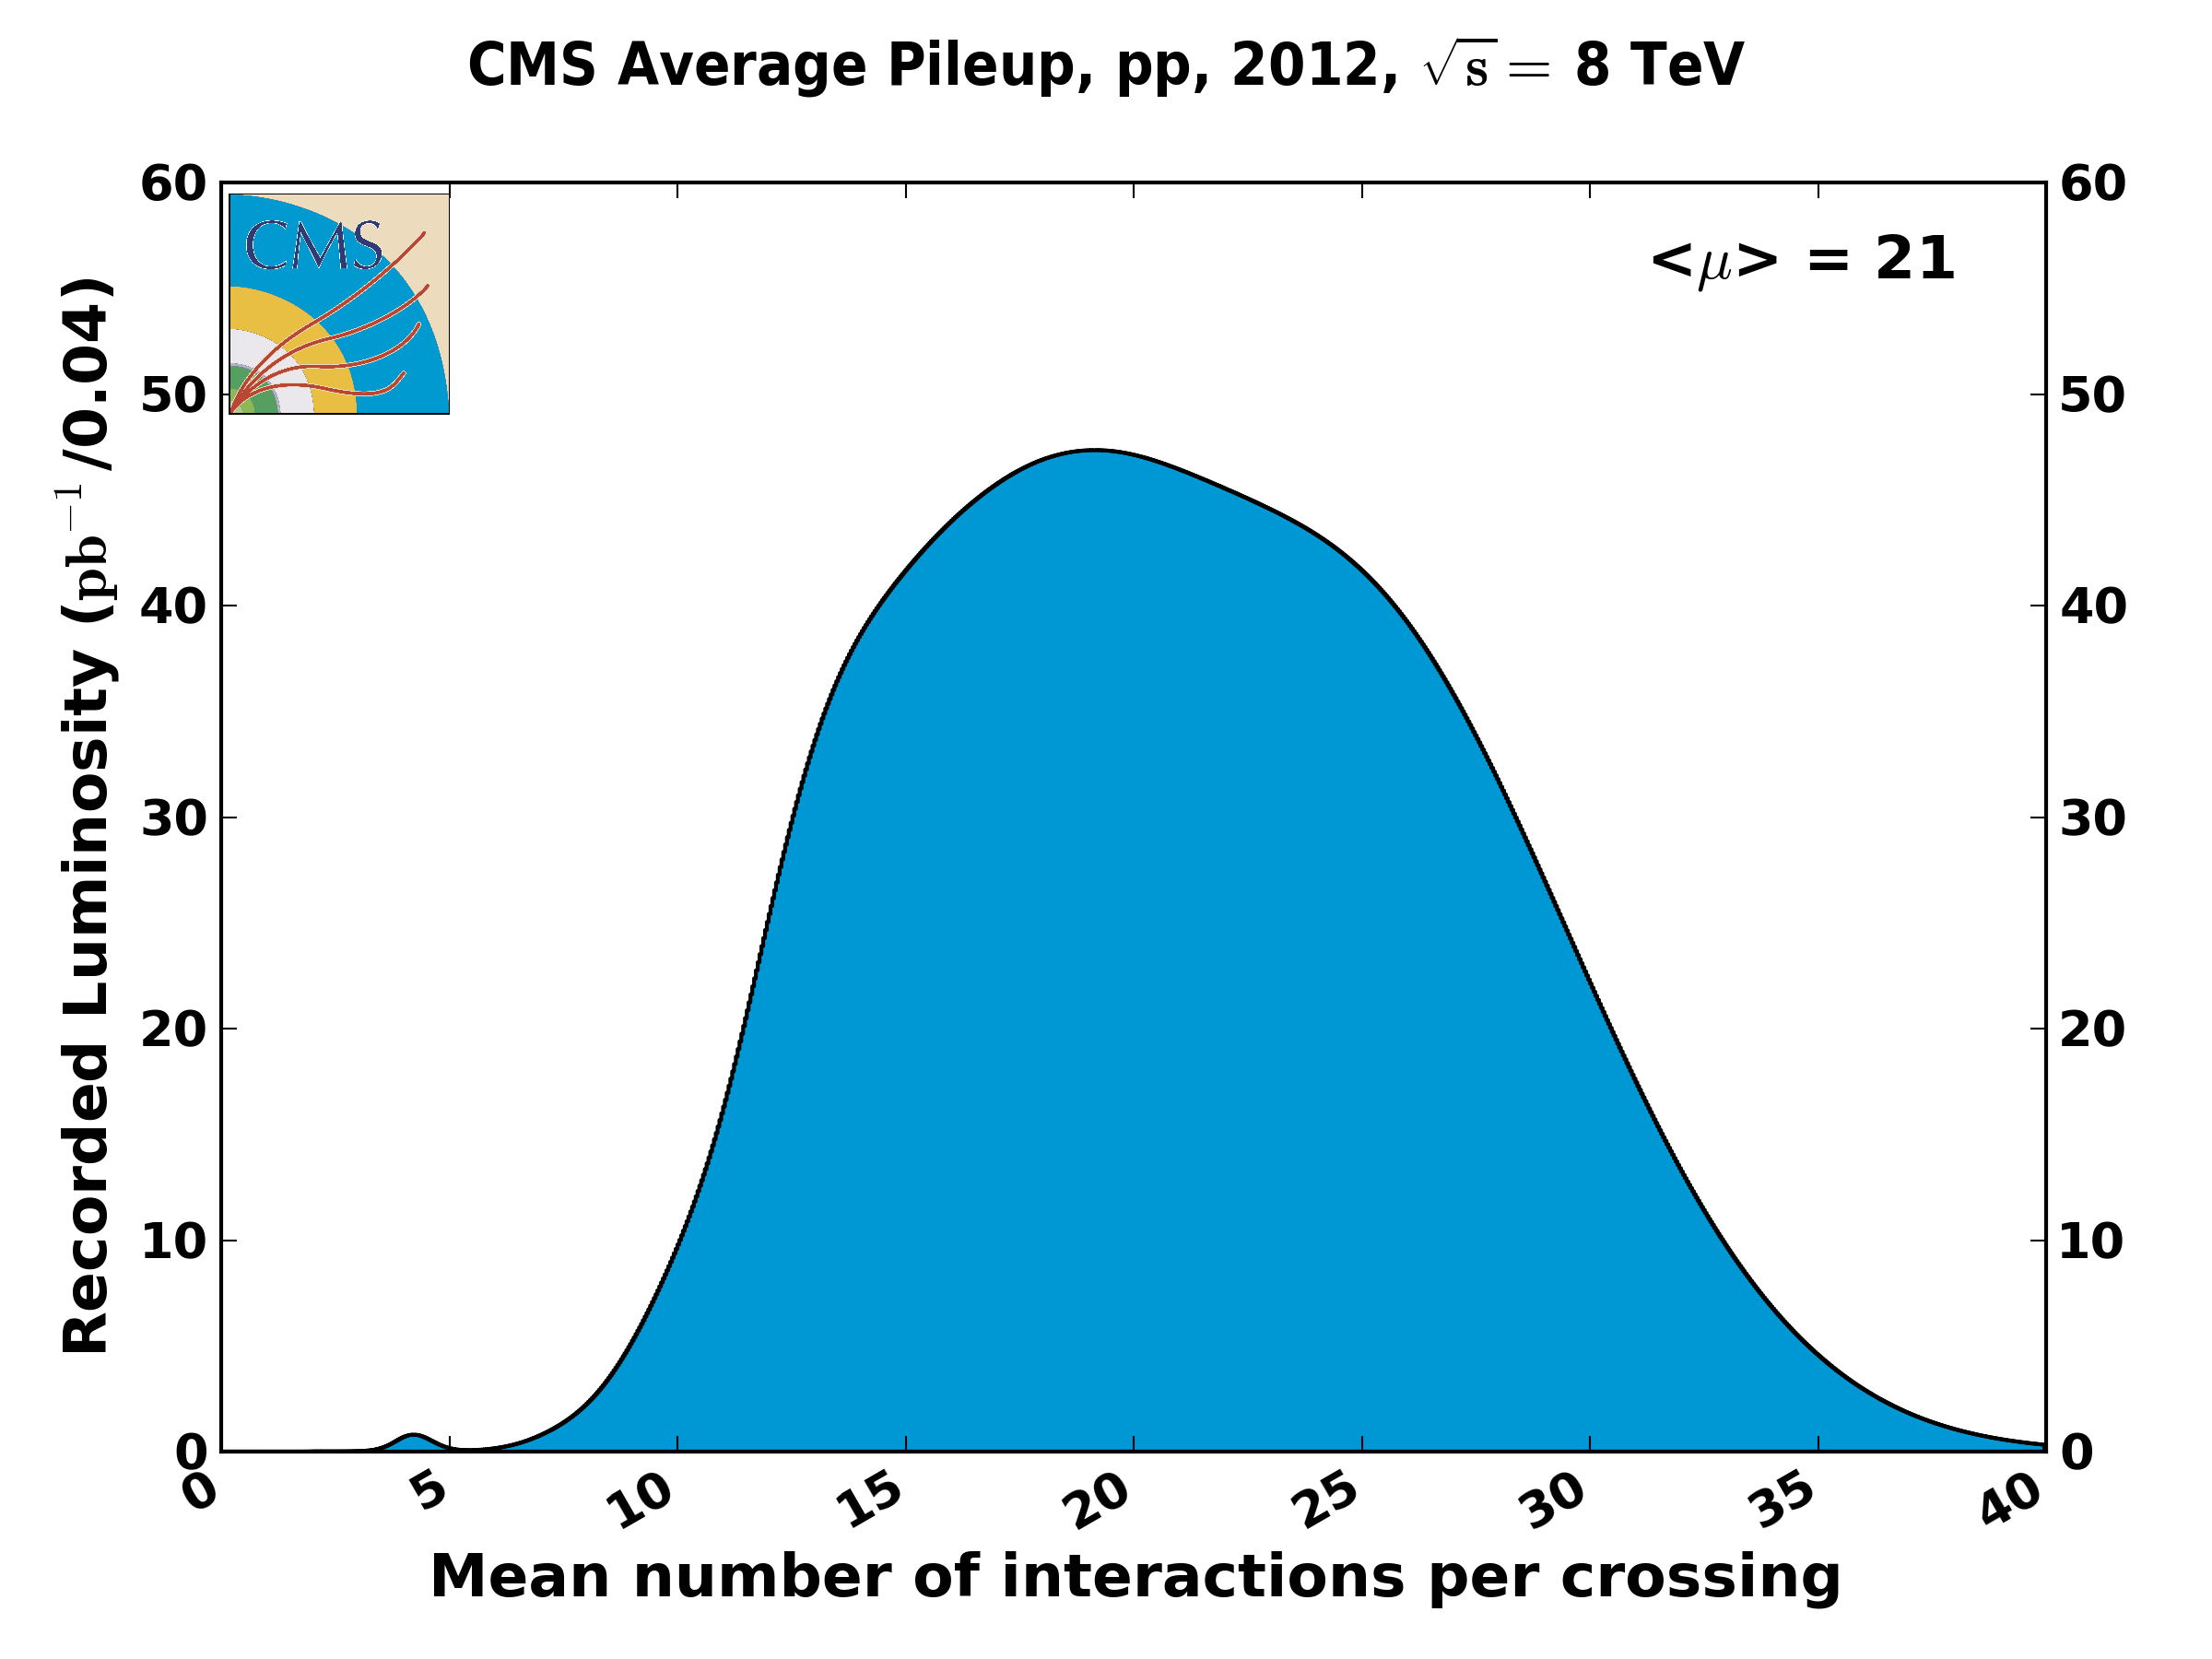
\includegraphics[width=0.8\textwidth]{ILC/figs/pileup_pp_2012.png}
    \caption{Distribution du nombre moyen d'interactions par croisement de faisceaux dans le détecteur CMS en 2012 \cite{cmslumiplot}.}
    \label{fig:cms-pileup}
  \end{center}
\end{figure}
La figure~\ref{fig:cms-pileup} montre la distribution du nombre moyen d'interactions par croisement de faisceaux dans le détecteur CMS en 2012. La valeur moyenne de cette distribution est $<\mu>=21$. Une amélioration du LHC en HL-LHC (High Luminosity Large Hadron Collider) entraînera une augmentation de cette valeur à environ $<\mu>=140$. Dans un collisionneur électron-positon, la principale source d’empilement provient de collision photon-photon \cite{physicsTDR}. Cependant la section efficace de ce phénomène est de quelques centaines de $nb$ alors qu'elle est d'environ 100 $mb$ pour des collisions proton-proton. Ainsi, pour l'ILC, une seule collision photon-photon produisant des hadrons, est attendu par croisement de faisceaux \cite{physicsTDR}. Une autre source d'empilement dans un collisionneur électron-positon correspond aux réactions de diffusion BhaBha ($e^+e^-\rightarrow e^+e^-$). De nombreuses paires $e^+e^-$ peuvent ainsi être créées mais seront pour la plupart émises proches du faisceau. 

Une autre contrainte à prendre en compte auprès des collisionneurs hadroniques est le niveau élevé de radiation. Les différents sous-détecteurs et particulièrement ceux qui sont très exposés doivent être résistants aux radiations. Ainsi, les trajectographes des expériences ATLAS et CMS, et le calorimètre électromagnétique des bouchons de CMS devront être remplacés pour le futur HL-LHC. 

Cependant, l'utilisation d'un accélérateur circulaire avec des hadrons permet d'atteindre des énergie beaucoup plus élevées qu'avec un accélérateur électron-positon. En effet, lorsqu'une particule chargée ultra-relativiste suit une trajectoire courbe, elle émet de l'énergie sous forme de rayonnement: le rayonnement synchrotron. L'énergie dissipée par rayonnement synchrotron est proportionnelle à $1/m^4$ ($m$ est la masse de la particule) et $1/R$ ($R$ est le rayon de courbure). Ainsi, l'énergie dissipée par rayonnement dans un collisionneur électron-positon est $10^{13}$ fois plus élevée que pour un collisionneur proton-proton. 

Pour atteindre les énergies suffisantes pour étudier le boson de Higgs ($\sqrt(s)\approx250~GeV$) avec un collisionneur leptonique électron-positon, plusieurs options sont envisagées. La première est un collisionneur linéaire pour lequel l'énergie dissipée par rayonnement synchrotron est nulle. Cependant, avec un accélérateur linéaire, les particules ne peuvent être accélérées qu'une seule fois. Le gradient d'accélération doit donc être très élevé pour conserver une taille de l'expérience "raisonnable". De plus, à la différence des accélérateurs circulaires, les particules n'ayant pas interagi après un croisement de faisceaux sont perdues. La deuxième option envisage un accélérateur circulaire de 50 à 70 $km$ (CEPC: Circular Electron Positron Collider) ou 80 à 100 $km$ (FCC: Futur Circular Collider) de périmètre. Ces options permettraient aussi d'envisager la transformation de ces machines en collisionneur hadronique pouvant atteindre des énergies de l'ordre de 100 $TeV$. Cependant, au contraire d'un accélérateur linéaire, l'énergie atteinte avec un tel collisionneur circulaire ne pourrait pas dépasser 400 $GeV$ dans le centre de masse. Une dernière option pourrait être un collisionneur circulaire produisant des collisions muon-anti-muon. L'énergie dissipée par rayonnement serait $\frac{m_{e}^4}{m_{\mu}^4}\approx5.5\times10^{-10}$ fois plus faible que pour un collisionneur électron-positon. Cependant le temps de vie des muons ($\tau_{\mu}=2.20\times10^{-6}~s$) compliquerait la réalisation d'une telle machine.

Le dernier avantage majeur des collisionneurs leptoniques est la possibilité d'utiliser des faisceaux polarisés. La polarisation correspond au taux de particules du faisceau, dont le spin est aligné avec le sens de propagation de ces particules. Dans un collisionneur électron-positon, les processus dominants sont des annihilations (voie $s$) et des diffusions (voies $t$ et $u$). Le spin de la particule échangée dans ces processus est corrélé aux hélicités (projection du spin sur l'axe de propagation) des particules incidentes. Ainsi, l'utilisation de faisceaux polarisés pourrait augmenter considérablement le taux de production d'un signal et aussi supprimer efficacement des bruits de fond. Par exemple, à $\sqrt{s}=500~GeV$, avec des faisceaux non polarisés, la réaction $e^+e^-\rightarrow W^+W^-$ a une section efficace de 6.2 $pb$. Avec une polarisation $(P_e^{-},P_e^{+})=(80\%,0\%)$, la section efficace de cette réaction est 1.2 $pb$ \cite{polarised_elec_beam}.

Ces différents avantages (énergie bien définie, propreté des événements, polarisation des faisceaux) font que les collisionneurs leptoniques constituent des machines très intéressantes pour effectuer des mesures de haute précision. Dans le cadre du TDR (Technical Design Report) de l'ILC \cite{physicsTDR}, ont été réalisées des projections sur les mesures des valeurs de couplages entre les différentes particules et le boson de Higgs. Le tableau~\ref{tab.higgs-coupling} présente les précisions attendues sur ces valeurs de couplages pour le LHC et pour différents scénarios de l'ILC (cf. section~\ref{sec.phys.program}). 
\begin{table}[!ht]
  \begin{center}
    \begin{tabular}{c|c|c|c|c}
      \rowcolor{black!20!white} Mode & LHC & ILC(250) & ILC(500) & ILC(1000)\\
      \hline
      \rowcolor{black!5!white}$WW$ & $4.1\%$ & $1.9\%$ & $0.24\%$ & $0.17\%$ \\
      \rowcolor{black!5!white}$ZZ$ & $4.5\%$ & $0.44\%$ & $0.30\%$ & $0.27\%$ \\
      \rowcolor{black!5!white}$bb$ & $13.6\%$ & $2.7\%$ & $0.94\%$ & $0.69\%$ \\
      \rowcolor{black!5!white}$gg$ & $8.9\%$ & $4.0\%$ & $2.0\%$ & $1.4\%$ \\
      \rowcolor{black!5!white}$\gamma\gamma$ & $7.8\%$ & $4.9\%$ & $4.3\%$ & $3.3\%$ \\
      \rowcolor{black!5!white}$\tau^+\tau^-$ & $11.4\%$ & $3.3\%$ & $1.9\%$ & $1.4\%$ \\
      \rowcolor{black!5!white}$c\bar c$ & $ $ & $4.7\%$ & $2.5\%$ & $2.1\%$ \\
      \rowcolor{black!5!white}$t\bar t$ & $15.6\%$ & $14.2\%$ & $9.3\%$ & $3.7\%$ \\
      \rowcolor{black!5!white}$\mu^+\mu^-$ & $ $ & $ $ & $ $ & $16\%$ \\
      \rowcolor{black!5!white}$self$ & $ $ & $ $ & $104\%$ & $26\%$ \\
      \hline
      \rowcolor{black!5!white}$BR(invis.)$ & $< 9\%$ & $< 0.44\%$ & $< 0.30\%$ & $< 0.26\%$ \\
      \rowcolor{black!5!white}$\Gamma_T (h)$ & $20.3\%$ & $4.8\%$ & $1.6\%$ & $1.2\%$ \\
    \end{tabular}
  \end{center}  
  \caption{Précision attendue pour les couplages de différentes particules au boson de Higgs. Pour les modes de désintégration du Higgs en signal invisible, une limite supérieure est donnée avec un taux de confiance à 95$\%$. Les quatre colonnes présentent les précisions attendues pour le LHC avec une luminosité de 300 $fb^{-1}$; l'ILC à 250 $GeV$ avec 250 $fb^{-1}$; l'ILC à 500 $GeV$ avec 500 $fb^{-1}$; et l'ILC à 1 $TeV$ avec 1000~$fb^{-1}$.}
  \label{tab.higgs-coupling}
\end{table}
Ces projections ont aussi été réalisées pour d'autres collisionneurs électron-positon. La figure~\ref{fig:kappa_factor} montre les projections sur la précision attendue sur les facteurs $\kappa_A$ pour les accélérateurs électron-positon et le LHC \cite{snowmass}. 
\begin{figure}[!h]
   \begin{center}
     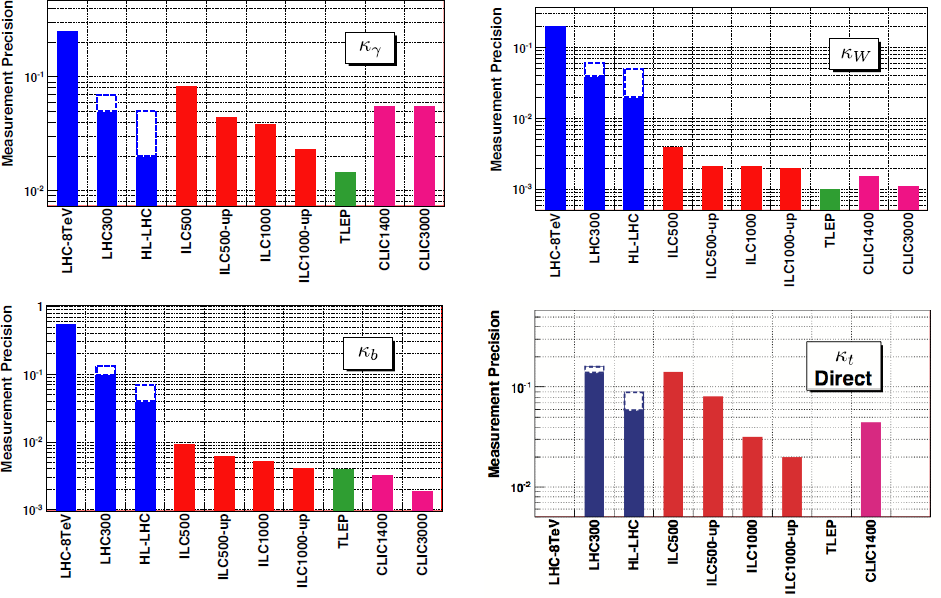
\includegraphics[width=1.0\textwidth]{ILC/figs/kappa_factor.png}
     \caption{Précision attendue sur les facteurs $\kappa_{\gamma}$, $\kappa_{W}$, $\kappa_{b}$ et $\kappa_{t}$ au LHC et ses différentes versions, pour plusieurs scénarios de l'ILC et pour les accélérateurs TLEP et CLIC \cite{snowmass}.}
     \label{fig:kappa_factor}
   \end{center}
\end{figure}
Les facteurs $\kappa_A$ sont définis par:
\begin{equation}
  \kappa_A=\frac{g_{HA\bar{A}}}{g_{HA\bar{A},SM}}
\end{equation}
où $g_{HA\bar{A}}$ correspond aux valeurs de couplage entre le boson de Higgs et les particules du modèle standard (fermions ou bosons vecteurs), et $g_{HA\bar{A},SM}$ aux valeurs de couplage prédites par le modèle standard. Le tableau~\ref{tab.higgs-coupling} et la figure~\ref{fig:kappa_factor} résument l'intérêt de la construction d'un collisionneur leptonique pour succéder au LHC et pour tester avec une grande précision le modèle standard.

\section{Le Collisionneur Linéaire International}
\begin{figure}[!ht]
  \begin{center}
    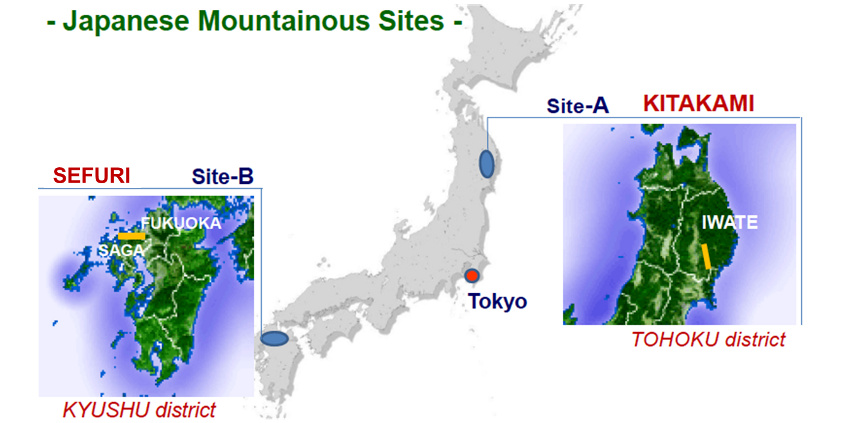
\includegraphics[width=0.75\textwidth]{ILC/figs/japanese_sites.jpg}
    \caption{Les deux sites candidats pour accueillir l'ILC au Japon.}
    \label{fig:japanese_sites}
  \end{center}
\end{figure}
Le Collisionneur Linéaire International (ILC) est un projet de collisionneur linéaire électron-positon avec une énergie dans le centre de masse comprise entre 200 et 500 $GeV$, avec la possibilité d'atteindre 1 $TeV$ en doublant la  longueur des accélérateurs principaux. Ce projet est né au début des années 2000 (premier workshop ILC en 2004 à KEK au Japon) et correspond aujourd'hui au projet de collisionneur leptonique le plus mature pour succéder au LHC. Si plusieurs pays ont semblé vouloir accueillir l'ILC, le Japon est celui qui a montré le plus d'intérêts. Des études pour accueillir une telle expérience ont été réalisées sur deux sites au Japon. Le site Iwate (cf. figure~\ref{fig:japanese_sites}) sous la montagne de Kitakami au nord de Tokyo a finalement été choisi. La décision finale concernant la construction de l'ILC pourrait intervenir en 2016. 

\subsection{Le complexe d'accélérateurs de l'ILC}
\begin{figure}[!ht]
  \begin{center}
    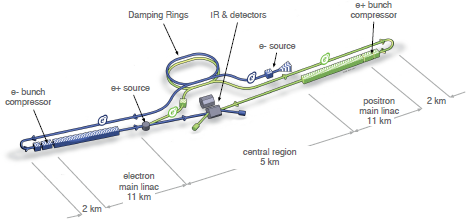
\includegraphics[width=1.0\textwidth]{ILC/figs/ilc-scheme.png}
    \caption{Schéma descriptif du complexe d'accélération de l'ILC.}
    \label{fig:ilc-scheme}
  \end{center}
\end{figure}
La figure~\ref{fig:ilc-scheme} présente un schéma du complexe d'accélération de l'ILC. Il indique les principaux sous systèmes du complexe \cite{introTDR}:
\begin{itemize}
\item une source d'électrons polarisés;
\item une source de positons polarisés;
\item deux anneaux de stockage ($Dumping~Rings$) des électrons et des positons, de 3.2 $km$ de circonférence;
\item deux accélérateurs linéaires principaux de 11 km basés sur la technologie de cavité radiofréquence supraconductrice (1.3 $GHz$) permettant d'obtenir un gradient moyen d'accélération de 31.5 $MV/m$;
\item deux systèmes de distribution du faisceau permettant des collisions avec un angle de 14 $mrad$ entre les deux faisceaux.
\end{itemize}
La chaîne d'accélération conduisant aux collisions électron-positon est la suivante. Premièrement, les électrons polarisés sont produits avec un laser illuminant une cible semi-conductrice en arséniure de gallium ($GaAs$). Ces électrons sont ensuite accélérés jusqu'à 5 $GeV$ et stockés dans leur anneau de stockage. Puis des électrons sont extraits, transférés dans leur accélérateur principal et accélérés jusqu'à environ 150 $GeV$. Ce faisceau d'électrons traverse ensuite un onduleur de 147 $m$, dans lequel des photons sont émis avec une énergie comprise entre 10 et 30 $MeV$. Ces photons sont ensuite dirigés vers une cible à base de titane avec une épaisseur correspondant à 0.4 longueur d'interaction. Les photons interagissent et créent des paires électron-positon. Les positons sont alors séparés des électrons et des photons restants, accélérés jusqu'à 5 $GeV$ puis conduits dans leur anneau de stockage. La machine est alors prête à produire des collisions électron-positon. Les électrons et les positons sont conduits dans leurs accélérateurs principaux. Les paquets sont d'abord comprimés puis accélérés dans les cavités radiofréquences supraconductrices.

\begin{figure}[!h]
  \begin{center}
    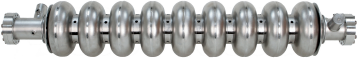
\includegraphics[width=1.0\textwidth]{ILC/figs/rf-cav.png}
    \caption{Photographie d'une cavité radiofréquence supraconductrice en niobium utilisée pour accélérer les électrons et les positons pour l'ILC.}
    \label{fig:rf-cav}
  \end{center}
\end{figure}
La figure~\ref{fig:rf-cav} présente une photographie d'une cavité qui sera utilisée pour l'ILC. Après 11 $km$ d'accélérations, les systèmes de distribution du faisceau entraînent les électrons et les positons jusqu'au point de collision. Ce système gère aussi plusieurs fonctions importantes, comme la réduction du halo du faisceau afin de réduire les bruits de fond (collisions photon-photon) dans les détecteurs. Cet accélérateur pourra atteindre une luminosité d'environ~$2\times10^{34}~cm^{-2}s^{-1}$ ($5\times10^{34}~cm^{-2}s^{-1}$ pour la version à 1 $TeV$). Il délivrera du faisceau pendant 0.95 $ms$ toute les 200 $ms$ ($\approx 5 Hz$). Pendant ces 0.95 $ms$, les paquets d'électron et de positons, espacés de 554 $ns$, rentreront en collision. Le tableau~\ref{tab.ilc-params} présente les valeurs des principaux paramètres du collisionneur ILC en fonction des différentes étapes de la machine. 
\begin{table}[!ht]
  \begin{center}
    \begin{tabular}{>{\centering}m{7cm}|c|c|c|c}
      \rowcolor{black!20!white}$\sqrt{s}$ & $GeV$ & $250$ & $500$ & $1000$ \\
      \hline
      \rowcolor{black!5!white}Taux de collision & $Hz$ & $5$ & $5$ & $4$ \\
      \rowcolor{black!5!white}Nombre de paquets par linac & $ $ & $1312$ & $1312$ & $2450$ \\
      \rowcolor{black!5!white}Nombre de particules par paquets & $\times 10^{10}$ & $2.0$ & $2.0$ & $1.74$ \\
      \rowcolor{black!5!white}Séparation entre les paquets & $ns$ & $554$ & $554$ & 366 \\
      \rowcolor{black!5!white}$ $ & $ $ & $ $ & $ $ & $ $ \\
      \rowcolor{black!5!white}Gradient d'accélération & $MVm^{-1}$ & $31.5$ & $31.5$ & $38.2$\\
      \rowcolor{black!5!white}$ $ & $ $ & $ $ & $ $ & $ $ \\
      \rowcolor{black!5!white}Polarisation des électrons & $\%$ & $80$ & $80$ & $80$ \\
      \rowcolor{black!5!white}Polarisation des positons & $\%$ & $30$ & $30$ & $20$ \\
      \rowcolor{black!5!white}$ $ & $ $ & $ $ & $ $ & $ $ \\
      \rowcolor{black!5!white}Luminosité & $\times 10^{34} cm^{-2} s^{-1}$ & $0.75$ & $1.8$ & $4.9$ \\
      \rowcolor{black!5!white}Taille horizontale du faisceau au point d'interaction & $nm$ & $729$ & $474$ & $481$ \\
      \rowcolor{black!5!white}Taille verticale du faisceau au point d'interaction & $nm$ & $7.7$ & $5.9$ & $2.8$ \\
    \end{tabular}
  \end{center}  
  \caption{Tableau récapitulatif des principales caractéristiques de l'ILC.}
  \label{tab.ilc-params}
\end{table}

\subsection{Les détecteurs de l'ILC}
Avec un collisionneur linéaire, il ne peut y avoir qu'un seul point de d'interaction. Cependant, afin éviter des biais expérimentaux et pour confirmer d'éventuels résultats, deux détecteurs sont à l'étude pour l'ILC. Ces deux détecteurs seront construits sur une plate-forme mobile et enregistreront tour à tour des données. De plus, auprès des détecteurs de l'ILC, la nouvelle approche de suivi des particules (PFA: Particle Flow Algorithm) pour mesurer l'énergie des jets sera utilisée. Cette approche consiste à utiliser le sous-détecteur le plus adapté pour mesurer l'énergie des particules dans les jets. Ainsi, l'énergie des particules chargées, qui représente en moyenne 65$\%$ de l'énergie d'un jet, sera déterminée en mesurant leur courbure dans le trajectographe. L'énergie des photons (en moyenne 25$\%$ de l'énergie d'un jet) sera mesurée avec le calorimètre électromagnétique. Enfin, l'énergie des hadrons neutres (en moyenne 10$\%$ de l'énergie d'un jet) sera mesurée dans les calorimètres. 
\begin{figure}[!h]
  \begin{center}
    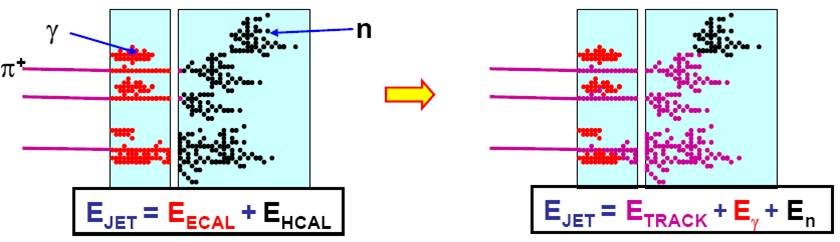
\includegraphics[width=1.0\textwidth]{ILC/figs/Particle_Flow_Paradigm.jpg}
    \caption{Schéma explicatif du principe de suivi des particules.}
    \label{fig:pfa-scheme}
  \end{center}
\end{figure}
La figure~\ref{fig:pfa-scheme} illustre le principe de mesure de l'énergie par suivi des particules. Traditionnellement, l'énergie des jets est déterminée en sommant l'énergie des dépôts dans les différents calorimètres. Avec le PFA, l'énergie reconstruite d'un jet $E_{jet}$ devient:
\begin{equation}
  E_{jet}=E_{traces}+E_{\gamma}+E_{neutres}
\end{equation}
où $E_{traces}$ est la somme des énergies des particules chargées, $E_{\gamma}$ la somme de l'énergie des photons et $E_{neutres}$ la somme de l'énergie des hadrons neutres. Le succès de cette approche réside dans la capacité à bien reconstruire la trajectoire des différentes particules dans tous les sous-détecteurs. Les dépôts dans les calorimètres doivent pouvoir être associés avec peu d'ambiguïté avec leur éventuelle trace dans le trajectographe. Pour obtenir un minimum d’ambiguïté, des calorimètres ultra-granulaires doivent être associés à un trajectographe avec un budget matière très faible. Le budget matière est défini comme le nombre de longueurs de radiation $X_0$ (cf. section~\ref{sec.x0} du chapitre~\ref{chap.shower}). Il faut, pour profiter au maximum de la précision de mesure de l'impulsion des particules chargées dans le trajectographe ($\frac{\Delta_p}{p^2}\approx 5\times10^{-5} (GeV/c)^{-1}$), éviter que ces particules interagissent de façon trop importante dans la partie centrale du détecteur (conversion des photons, début de gerbes électromagnétiques ou hadroniques). Une très haute granularité dans les calorimètres est une condition nécessaire pour réussir la séparation entre les dépôts énergétiques issus des particules chargées et ceux issus des particules neutres. 

\begin{figure}[!ht]
  \begin{center}
    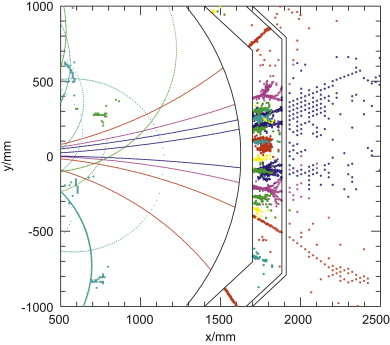
\includegraphics[width=.6\textwidth]{ILC/figs/pfa_ild.jpg}
    \caption{Exemple de reconstruction d'un jet de 100 $GeV$ issu de la désintégration d'un boson Z dans l'ILD.}
    \label{fig:pfa-example}
  \end{center}
\end{figure}
La figure~\ref{fig:pfa-example} montre un exemple de simulation d'événement avec un jet de 100 $GeV$ issu de la désintégration d'un boson Z en $u\bar u$ dans le Grand Détecteur International (ILD) avec une énergie de 200 $GeV$ dans le centre de masse \cite{pfaPandora}. Les différentes particules sont reconstruites, et le cas échéant, associées à une trace. 

Cependant, une très grande granularité pourrait entraîner une importante consommation électrique. Ainsi, la chaleur dissipée par ce grand nombre de canaux électroniques induirait du bruit dans les détecteurs. De plus, l'utilisation de systèmes de refroidissement actifs des sous-détecteurs augmenterait le budget matière entre ces détecteurs et dégraderait donc les performances des algorithmes de suivi de particules. Pour limiter la consommation et son bruit induit, les détecteurs de l'ILC devront mettre à profit le faible taux de collision (5 $Hz$). Les différents sous-détecteurs utiliseront une alimentation pulsée: les composants avec une forte consommation électrique devront automatiquement s'éteindre pendant les 199.05 $ms$ sans croisement de faisceaux. 

Pour répondre aux différentes contraintes imposées par l'ILC, deux collaborations travaillent au développement de deux détecteurs: le Grand Détecteur International (ILD: International Large Detector) et le Détecteur au Silicium (SiD: Silicon Detector). Ces deux détecteurs sont des détecteurs généralistes avec un trajectographe, un calorimètre électromagnétique et un calorimètre hadronique intégrés dans un aimant (solénoïde supraconducteur), puis des chambres à muons. Ces deux détecteurs ont été imaginés pour répondre à plusieurs critères basés sur les performances requises pour étudier les propriétés du boson de Higgs, comme sa masse, son auto-couplage, ses rapports de branchement, ou la découverte de particules supersymétriques. Le tableau~\ref{tab.ilc-det-perf} présente les performances requises des différents sous-détecteurs.
\begin{table}[!ht]
  \begin{center}
    \begin{tabular}{>{\centering}m{5cm} | >{\centering}m{6cm} | c }
      \hline
      \rowcolor{black!20!white} sous-détecteurs & Observable & Performance \\
      \hline
      \rowcolor{black!5!white} Trajectographe, \newline Chambre à muons & Résolution sur l'impulsion des particules chargées:\newline $\frac{\Delta_{p_t}}{p_t^2}$ & $5\times10^{-5}\ (GeV/c)^{-1}$\\
      \hline
      \rowcolor{black!5!white} Trajectographe, \newline Calorimètre & Résolution en énergie des jets:\newline $\dfrac{\Delta_{E}}{E}$ & $3-4\%$\\
      \hline
      \rowcolor{black!5!white} Vertex & Résolution spatiale & $3\ \mu m$\\
      \rowcolor{black!5!white} $ $ & Budget matière & $0.15\% X_0/plan$\\
      \rowcolor{black!5!white} $ $ & Rayon du premier plan & $\simeq 1.6\ cm$\\
    \end{tabular}
  \end{center}  
  \caption{Performances requises pour les sous-détecteurs des détecteurs de l'ILC.}
  \label{tab.ilc-det-perf}
\end{table}


\subsection{Le Grand Détecteur International ILD}
\begin{figure}[!ht]
  \begin{center}
    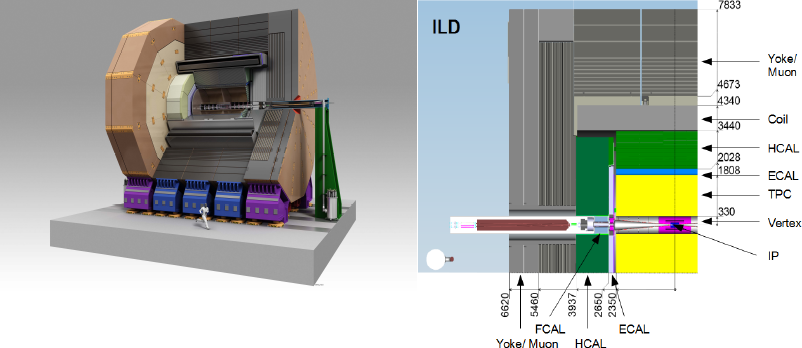
\includegraphics[width=1.0\textwidth]{ILC/figs/ild.png}
    \caption{Image artistique (à gauche) et vue en coupe d'un quadrant (à droite) du détecteur ILD.}
    \label{fig:ild-scheme}
  \end{center}
\end{figure}
Le Grand Détecteur International ILD a été imaginé pour répondre aux différentes contraintes imposées par l'ILC. Une variante de ce détecteur légèrement modifiée a aussi été proposée pour l'expérience Collisionneur Linéaire Compact (CLIC)~\cite{clic}. Même si des études portant sur l'optimisation de ce détecteur sont toujours en cours, un rapport (Detailed Baseline Detector) publié en 2013 au sein du rapport TDR (Technical Desin Report) de l'ILC, présente une version relativement mature de l'ILD \cite{detectorTDR}. La suite de cette section décrit le Grand Détecteur International en se basant sur ce rapport. Ce détecteur comporte un détecteur de vertex, suivi d'un système hybride comportant des détecteurs au silicium et une chambre à projection temporelle (TPC) puis des calorimètres. Cet ensemble est inséré dans un solénoïde fournissant un champ magnétique de 3.5 $T$. A l'extérieur de l'aimant, des chambres à muons sont insérées dans une culasse en fer pour canaliser le retour du champ magnétique. La figure~\ref{fig:ild-scheme} présente un schéma artistique de l'ILD et une vue en coupe de ce détecteur. 
\subsubsection{Le détecteur de vertex}
Le détecteur de vertex permet de reconstruire les vertex primaires d'interaction et les vertex secondaires issus de la désintégration de particules avec des courts temps de vie comme les mésons D ($c\tau_{D^{\pm}}=311.8\mu m$) et B ($c\tau_{B^{\pm}}=491.1\mu m$) \cite{pdg}. Pour l'ILD, le détecteur de vertex est constitué de trois couches cylindriques proches du point d'interaction (rayon de la première couche: 1.6 $cm$). Chaque couche est équipée sur chacune de ses faces d'un détecteur à pixels de silicium, ce qui permet d'avoir 6 points de mesure de la trajectoire des particules chargées dans ce détecteur. Plusieurs technologies de senseurs sont considérées pour équiper le détecteur de vertex. Pour chaque couche, le budget matière est équivalent à $0.30\% X_0/couche$ (ou $0.15\% X_0/plan$). La résolution spatiale ($\sigma$) est inférieure à 3 $\mu m$ pour le plan le plus proche du point d'interaction. Enfin, la couche la plus interne doit être capable de résister à une dose de l'ordre de 1 $kGy$ par an. Le tableau~\ref{tab.vtx-param} résume les paramètres des différents plans du détecteur de vertex de l'ILD.
\begin{table}[!ht]
  \begin{center}
    \begin{tabular}{c|c|c|c}
      \rowcolor{black!20!white} Plan & Rayon ($mm$) & $\sigma~(\mu m)$ \\
      \hline
      \rowcolor{black!5!white} $1$ & $16$ & $2.8$ \\
      \rowcolor{black!5!white} $2$ & $16$ & $6$ \\
      \hline
      \rowcolor{black!5!white} $3$ & $37$ & $4$ \\
      \rowcolor{black!5!white} $4$ & $39$ & $4$ \\
      \hline
      \rowcolor{black!5!white} $5$ & $58$ & $4$ \\
      \rowcolor{black!5!white} $6$ & $60$ & $4$ \\
    \end{tabular}
  \end{center}  
  \caption{Paramètres des différents plans du détecteur de vertex de l'ILD.}
  \label{tab.vtx-param}
\end{table}

\subsubsection{Les détecteurs au silicium}
Le trajectographe de l'ILD sera équipé de quatre détecteurs au silicium. Deux détecteurs seront insérés dans le tonneau: le SIT (Silicon Internal Tracker) entre le détecteur de vertex et la TPC; le SET (Silicon External Tracker) entre la TPC et le calorimètre électromagnétique. Deux autres détecteurs au silicium seront insérés dans les bouchons: le FTD (Forward Tracking Detector) entre le tube du faisceau et la TPC; le ETD (Endcap Tracking Detector) entre la TPC et le calorimètre électromagnétique. Les détecteurs SIT, SET et ETD permettent d'améliorer l'association des traces entre le détecteur de vertex et la TPC, et entre la TPC et le calorimètre électromagnétique en repérant précisément le point d'entrée et de sortie de la TPC. La détection des particules chargées est réalisée à l'aide de bandes croisées de silicium de 10 $cm$ de long et 50 $\mu m$ de large. L'intérêt du détecteur FTD est d'étendre la couverture angulaire de la TPC pour des angles faibles ($cos\theta>0.802$)\footnote{$\theta$ correspond à l'angle polaire dans un système de coordonnées $(z,\theta,\phi)$, régulièrement utilisé en physique des particules. $z$ correspond à l'axe du faisceau et $\phi$  à l'angle azimutal.}. La détection sera faite à l'aide de pixels de silicium. 

\subsubsection{La chambre à projection temporelle}
La chambre à projection temporelle constitue le principal détecteur du trajectographe de l'ILD. Une TPC est un détecteur gazeux permettant de reconstruire la trajectoire de particules chargées qui la traversent. Ces particules ionisent le mélange de gaz le long de leur trajectoire. Les charges ainsi produites dérivent, grâce à un champ électrique parallèle au faisceau pour l'ILD, vers les bouchons, puis subissent un processus de multiplication pour être détectées. 

Deux technologies sont envisagées pour effectuer le processus de multiplication et de détection: des GEM (Gas Electron Multiplier) ou des Micromegas. Pour la lecture des signaux, les deux options utilisent des carreaux de cuivre de $1\times6~mm^2$ couplées à l'utilisation d'une couche résistive. Cette technique permet d'étaler la charge sur plusieurs carreaux et ainsi d'obtenir une meilleure résolution spatiale en construisant le barycentre des charges. L'information 2D ($r,\phi$)\footnote{$r$ correspond à la distance par rapport à l'axe du faisceau.} ainsi obtenue permet de reconstruire la trajectoire de la trace en utilisant la vitesse de dérive des charges dans le gaz. L'utilisation d'une chambre à projection temporelle comporte plusieurs avantages pour un collisionneur leptonique. Les traces sont reconstruites avec un grand nombre de points ce qui permet de compenser une moins bonne résolution spatiale que celle peut obtenir un détecteur au silicium. Le budget matière d'une TPC est faible. Enfin, une TPC permet de réaliser de l'identification des particules en étudiant la perte d'énergie $dE/dx$. Le tableau~\ref{tab.tpc-params} présente les paramètres de la TPC de l'ILD.
\begin{table}[!ht]
  \begin{center}
    \begin{tabular}{c|c}
      \rowcolor{black!20!white} Paramètre & Valeur \\
      \hline
      \rowcolor{black!5!white} Rayon interne & $329~mm$ \\
      \rowcolor{black!5!white} Rayon externe & $1808~mm$ \\
      \rowcolor{black!5!white} Demi longueur & $2350~mm$ \\
      \rowcolor{black!5!white} Couverture angulaire & jusqu'à $cos\theta\approx0.98$ \\
      \rowcolor{black!5!white} Taille des carreaux de lecture & $1\times6~mm^2$ \\
      \hline
      \rowcolor{black!5!white} Résolution spatiale en $r\phi$ & $60-100~\mu m$ \\
      \rowcolor{black!5!white} Résolution spatiale en $rz$ & $0.4-1.4~mm$ \\
      \rowcolor{black!5!white} Résolution $dE/dx$ & $5\%$ \\
      \rowcolor{black!5!white} Résolution sur l'impulsion des traces & $10^{-4}~(GeV/c)^{-1}$ \\
    \end{tabular}
  \end{center}  
  \caption{Principaux paramètres de la chambre à projection temporelle de l'ILD~\cite{detectorTDR}.}
  \label{tab.tpc-params}
\end{table}

\begin{figure}[!ht]
  \begin{center}
    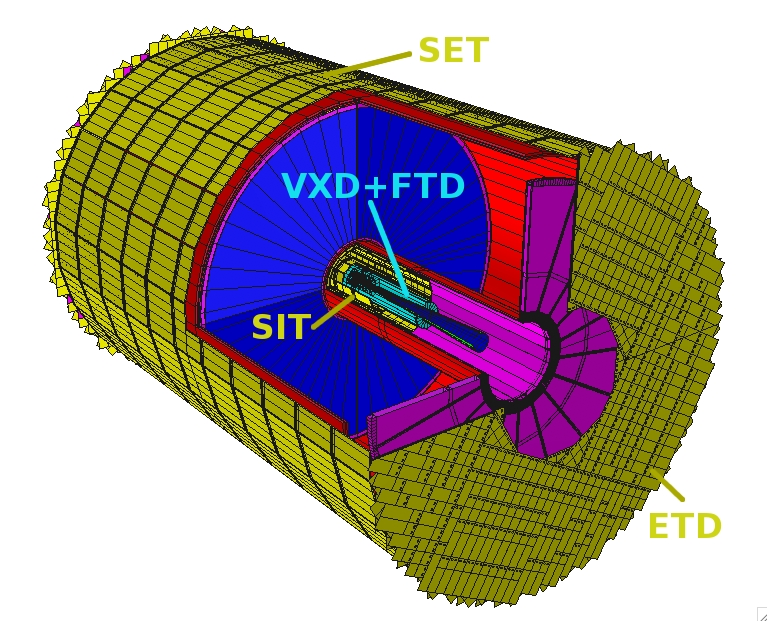
\includegraphics[width=.43\textwidth]{ILC/figs/Image_7b.jpg}
    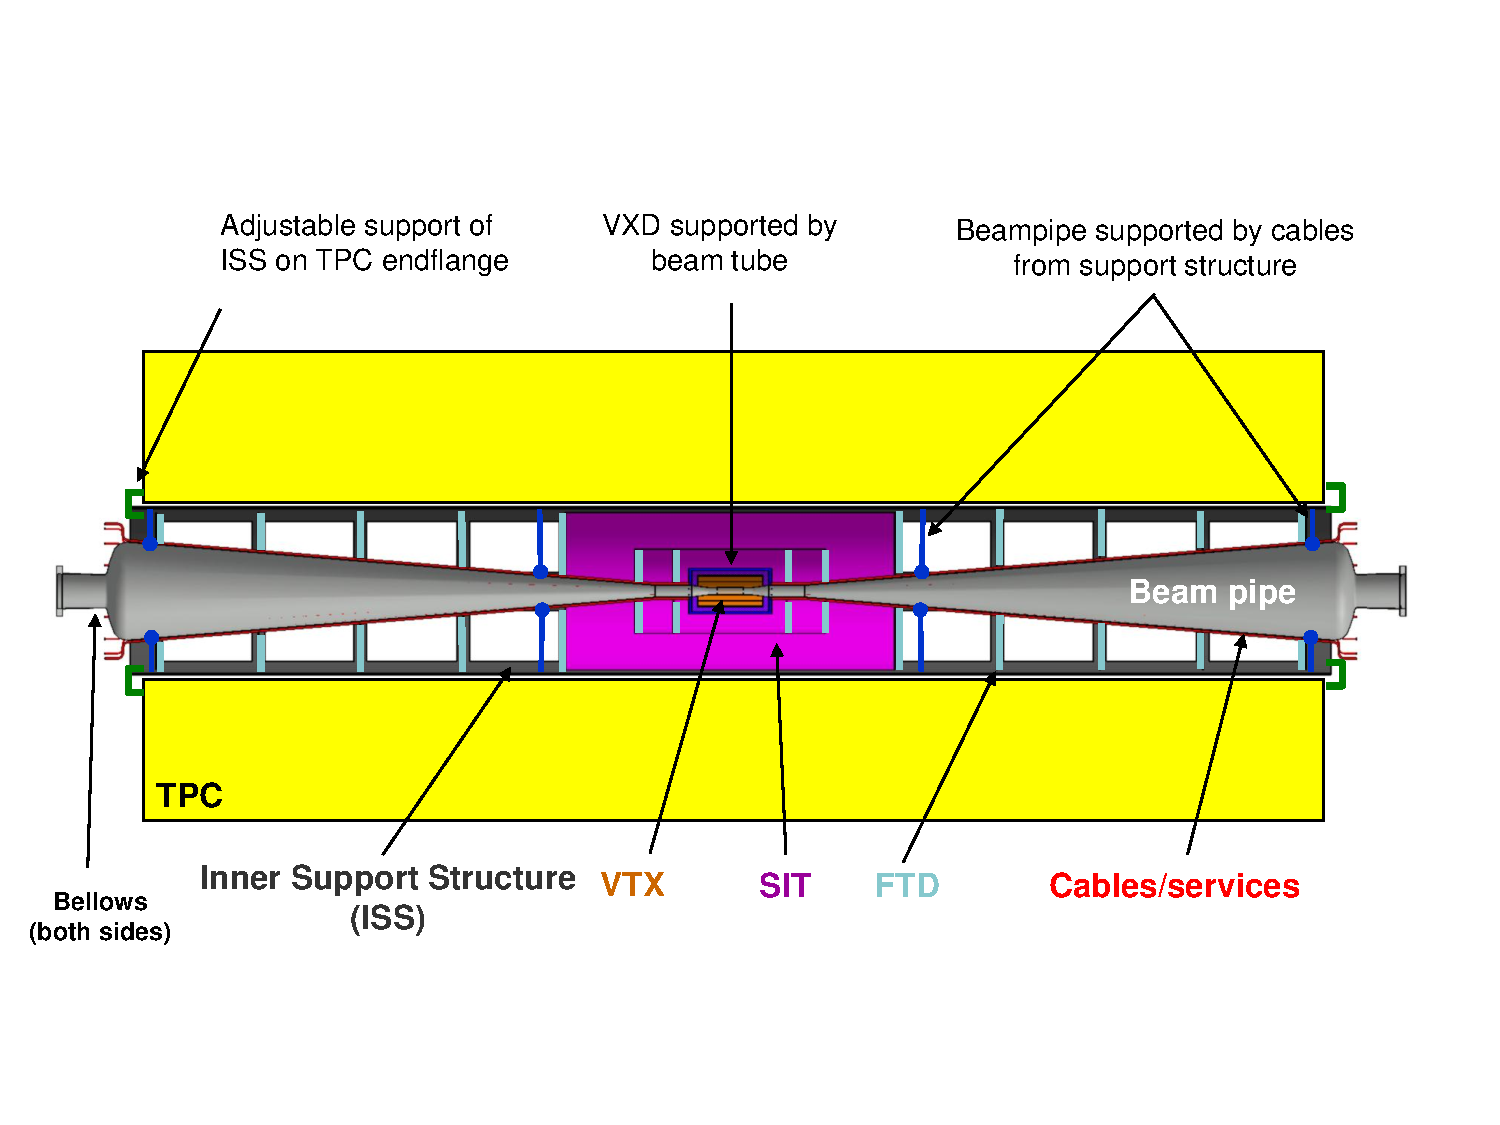
\includegraphics[width=.55\textwidth]{ILC/figs/ILd_inner.pdf}
    \caption{Image 3D (à gauche) et vue en coupe (à droite) du trajectographe de l'ILD et ses composants.}
    \label{fig:ild-traj}
  \end{center}
\end{figure}
La figure~\ref{fig:ild-traj} montre une image 3D et une vue en coupe du système de trajectographe de l'ILD et de ses composants.
\newpage
\subsubsection{Les calorimètres}
Les technologies, traditionnellement utilisées pour la calorimétrie, étaient plutôt optimisées pour obtenir la meilleure résolution en énergie possible. Pour les détecteurs de l'ILC, la capacité de séparation des différents dépôts énergétiques, couplée à une raisonnable résolution en énergie, a particulièrement influencé la conception des calorimètres. 
\begin{figure}[!h]
  \begin{center}
    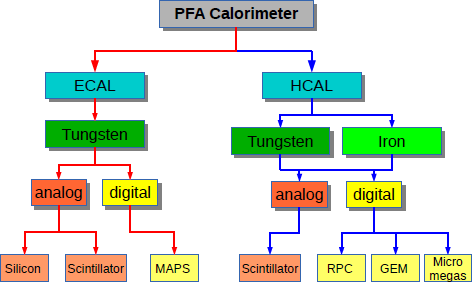
\includegraphics[width=.7\textwidth]{ILC/figs/pfaCalo.png}
    \caption{Les différents types de calorimètres ultra-granulaires pour l'application d'algorithmes de suivi de particules, envisagés pour les détecteurs de l'ILC.}
    \label{fig:calopfa}
  \end{center}
\end{figure}
La figure~\ref{fig:calopfa} recense les différentes technologies envisagées pour les calorimètres électromagnétiques et hadroniques de l'ILD. Toutes les options de calorimètres électromagnétiques et hadroniques proposent des calorimètres à échantillonnage. Les calorimètres à échantillonnage permettent, grâce à leur segmentation longitudinale, d'obtenir une image 3D des gerbes électromagnétiques et hadroniques. Le calorimètre électromagnétique utilisera des absorbeurs en tungstène tandis que le calorimètre hadronique utilisera de l'acier. Pour un détecteur auprès de l'accélérateur CLIC, le tungstène serait choisi comme absorbeur du calorimètre hadronique car l'énergie des jets serait plus élevée que pour l'ILC (cf. section~\ref{sec.clic} de ce chapitre). Le tableau~\ref{tab.caloParams} présente les principaux paramètres géométriques des calorimètres de l'ILD dans le tonneau. La plupart de ces paramètres sont susceptibles d'être modifiés afin d'optimiser les performances et le coût de l'ILD.
\begin{table}[!ht]
  \begin{center}
    \begin{tabular}{c|c|c}
      \rowcolor{black!20!white} $ $ & Paramètre & Valeur \\
      \rowcolor{black!5!white} ECAL & Rayon interne & $1843~mm$ \\
      \rowcolor{black!5!white} $ $ & Rayon externe & $2028~mm$ \\
      \rowcolor{black!5!white} $ $ & Nombre de couches actives & $30$ \\
      \rowcolor{black!5!white} $ $ & Taille des cellules & $5\times5~mm^2$ ou $5\times45~mm^2$\\
      \rowcolor{black!5!white} $ $ & Nombre de longueurs de radiation & $24X_0$ \\
      \hline
      \rowcolor{black!5!white} HCAL & Rayon interne & $2058~mm$ \\
      \rowcolor{black!5!white} $ $ & Rayon externe & $3410~mm$ \\
      \rowcolor{black!5!white} $ $ & Nombre de couches actives & $48$ \\
      \rowcolor{black!5!white} $ $ & Taille des cellules & $30\times30~mm^2$ ou $10\times10~mm^2$ \\
      \rowcolor{black!5!white} $ $ & Nombre de longueurs d'interaction & $6\lambda_I$ \\
    \end{tabular}
  \end{center}  
  \caption{Principaux paramètres géométriques des calorimètres de l'ILD~\cite{detectorTDR}.}
  \label{tab.caloParams}
\end{table}

\subsubsection{Le calorimètre électromagnétique}
La motivation principale pour le calorimètre électromagnétique de l'ILD est l'identification et la séparation des photons et des électrons, ainsi que la mesure précise de l'énergie des photons. Plusieurs options sont étudiées au sein de la collaboration CALICE pour équiper le calorimètre électromagnétique de l'ILD. 

La première option (SiECAL) utilise des galettes de silicium comme partie active. Ces galettes ont une segmentation transverse de $5\times5~mm^2$ et une épaisseur de 330 $\mu m$. Avec cette segmentation, le calorimètre électromagnétique du détecteur final comptera environ 100 millions de canaux électroniques. Un prototype utilisant cette technologie a été construit au sein de la collaboration CALICE et testé sur faisceau. Ce prototype a une segmentation transverse de $10\times10~mm^2$. La résolution obtenue avec le prototype est $\sigma_E/E=16\%/\sqrt{E}\oplus1.1\%$ \cite{siw-ecal}. 

Une deuxième option (ScEcaL) utilise des bandes croisées de plastique scintillant de $5\times45~mm^2$. Cette option permettrait d'obtenir une segmentation effective de $5\times5~mm^2$ et de fortement diminuer le nombre de canaux électroniques. Le prototype CALICE-ScECAL, avec une segmentation transverse de $45\times10~mm^2$, a une résolution en énergie $\sigma_E/E=13.5\%/\sqrt{E}\oplus3.5\%$~\cite{calice-scecal}. Cependant, avec une telle technologie, la reconstruction et la séparation des dépôts pourraient s'avérer compliquées notamment pour des jets denses. 

Pour ces deux options, des études d'optimisation sont toujours en cours pour réduire le coût de l'expérience finale tout en respectant les performances requises pour les détecteurs de l'ILC (cf. tableau~\ref{tab.ilc-det-perf}). Le rayon interne du calorimètre électromagnétique, le nombre de couches, la longueur des bandes de scintillateur font partie des principales sources d'optimisation. Parmi les études d'optimisation, une option de calorimètre hybride avec des couches utilisant les galettes de silicium alternées avec des couches de bandes de scintillateur est aussi envisagée. 
\begin{figure}[!ht]
  \begin{center}
    \subfigure[]{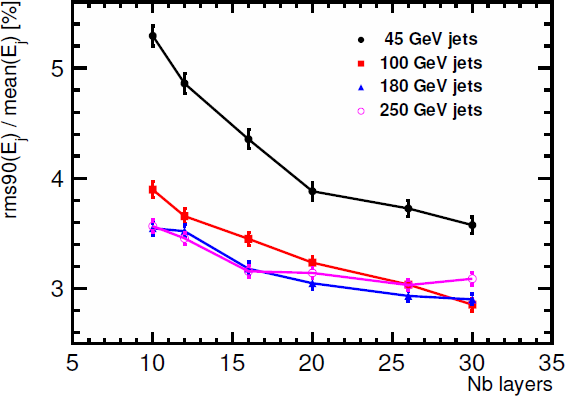
\includegraphics[width=0.55\textwidth]{ILC/figs/siecalNLayer.png}}
    \subfigure[]{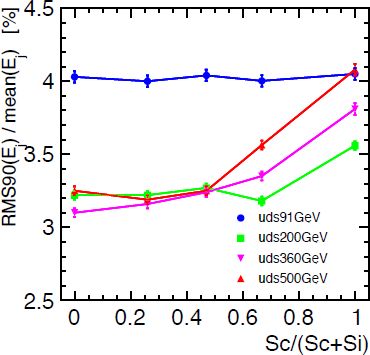
\includegraphics[width=0.44\textwidth]{ILC/figs/siscecalProp.png}}
    \caption{(a): Résolution en énergie de jets de 45, 100, 180 et 250 $GeV$ en fonction du nombre de couches actives du calorimètre électromagnétique (option SiECAL). (b): Résolution en énergie pour des événement di-jets à 91, 200, 360 et 500 $GeV$ dans le centre de masse en fonction de la proportion du nombre de couches avec des scintillateurs \cite{detectorTDR}.}
    \label{fig:ecalOpt}
  \end{center}
\end{figure}
La figure~\ref{fig:ecalOpt}(a) montre la résolution en énergie des jets en fonction du nombre de couches actives avec des galettes de silicium. La taille du calorimètre et son budget matière restent inchangés. La dégradation de la résolution en passant de 30 à 20 couches est environ de 10$\%$.  En réduisant encore le nombre de couches, la détérioration est plus significative, particulièrement à plus basse énergie. La figure~\ref{fig:ecalOpt}(b) montre la résolution en énergie d'événements di-jets en fonction de la proportion du nombre de couches avec des bandes de scintillateur. A basse énergie, la résolution n'est pas influencée par le nombre de couches avec des scintillateurs. A plus haute énergie, une détérioration significative est observée lorsque la proportion du nombre de couches de scintillateur est supérieure à 50$\%$.

Enfin, notons qu'une option de calorimètre utilisant des détecteurs MAPS (Monolitic Active Pixel Sensor) avec une lecture digitale pourrait permettre d'obtenir une segmentation transverse de l'ordre de $50\times50~\mu m^2$. Cette option est tout de même moins mature que les deux précédentes. 

\subsubsection{Le calorimètre hadronique}
Le principale rôle du calorimètre hadronique de l'ILD sera de séparer correctement les dépôts énergétiques laissés par les hadrons chargés et neutres, et de mesurer précisément l'énergie des hadrons neutres. Rappelons que l'énergie des  hadrons neutres constitue en moyenne 10$\%$ de l'énergie totale d'un jet. Plusieurs options sont proposées par la collaboration CALICE pour le calorimètre hadronique du détecteur ILD. Les différentes options sont des calorimètres à échantillonnage avec 48 couches actives insérées entre des plaques d'acier. 

Une première option (AHCAL) utilise des tuiles scintillantes en plastique comme milieu actif. Ces tuiles ont une segmentation transverse de $3\times3~cm^2$. Un prototype physique a été construit en 2007 \cite{ahcal-construction}. Ce prototype est légèrement différent du calorimètre proposé pour l'ILD: il contient des tuiles de $3\times3~cm^2$ dans sa région centrale ($30\times30~cm^2$), de $6\times6~cm^2$ puis $12\times12~cm^2$ à l'extérieur. La résolution en énergie intrinsèque pour des gerbes hadroniques mesurée avec ce détecteur est $\sigma_E/E=58\%/\sqrt{E}\oplus1.6\%$ \cite{ahcal-energy}. Cette résolution devient environ $\sigma_E/E=45\%/\sqrt{E}$ en utilisant des techniques de compensation pour égaliser les réponses hadronique et électromagnétique du calorimètre. 

Une deuxième option (SDHCAL) utilise des chambres à plaque résistive de verre (GRPC) comme milieu actif avec une lecture semi-digitale. Ce concept de calorimètre et les résultats obtenus avec un prototype seront présentés dans le chapitre~\ref{chap.sdhcal}. D'autres détecteurs gazeux, comme les Micromegas et les GEM pourraient être des alternatives aux GRPC si les coûts de production de ces détecteurs baissent significativement. 

Plusieurs option de géométrie du calorimètre hadronique dans le tonneau de l'ILD sont aussi étudiées.
\begin{figure}[!ht]
  \begin{center}
    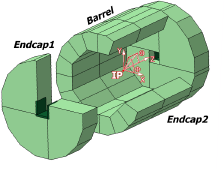
\includegraphics[width=0.48\textwidth]{ILC/figs/hcal1.png}
    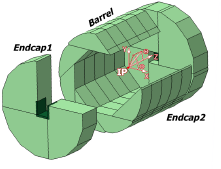
\includegraphics[width=0.48\textwidth]{ILC/figs/hcal2.png}
    \caption{Les différentes géométries envisagées pour le calorimètre hadronique de l'ILD.}
    \label{fig:hcalDesign}
  \end{center}
\end{figure}
La figure~\ref{fig:hcalDesign} présente les deux options de géométrie pour le calorimètre hadronique. La première structure (à gauche sur la figure~\ref{fig:hcalDesign}) est imaginée pour accueillir le calorimètre AHCAL et présente une géométrie standard où le tonneau est divisé en deux sections en $z$ et huit sections en $\phi$, pour un total de 32 modules indépendants. La deuxième option (à droite dur la figure~\ref{fig:hcalDesign}) est prévue pour l'intégration du calorimètre SDHCAL. Cette structure est optimisée pour réduire les zones non instrumentées du détecteur. Le tonneau est divisé en cinq roues, qui sont constituées de huit modules indépendants. 

\subsubsection{Les calorimètres vers l'avant}
En plus des calorimètres dans le tonneau et les bouchons, trois autres systèmes de calorimètres sont proposés pour équiper les régions proches du faisceau (calorimètres vers l'avant). Le LumiCal sert à mesurer la luminosité. Le BeamCal sera utilisé pour mesurer le bruit photon-photon. Ces deux calorimètres permettront d'étendre la couverture angulaire du calorimètre électromagnétique. Le LHCAL est une extension du calorimètre hadronique pour des angles faibles. La tableau~\ref{tab.forwardCalo} indique les couvertures angulaires de ces trois calorimètres.
\begin{table}[!ht]
  \begin{center}
    \begin{tabular}{c|c}
      \rowcolor{black!20!white} Calorimètre & Couverture angulaire $\Delta\theta$ ($mrad$) \\
      \rowcolor{black!5!white} LumiCal & $[31;77]$ \\
      \rowcolor{black!5!white} BeamCal & $[5;40]$ \\
      \rowcolor{black!5!white} LHCAL & $[31;77]$ \\
    \end{tabular}
  \end{center}
  \caption{Couverture angulaire des calorimètres de l'ILD disposés vers l'avant~\cite{detectorTDR}.}
  \label{tab.forwardCalo}
\end{table}

\subsubsection{Les chambres à muons}
Les sous-détecteurs que nous venons de décrire sont insérés dans un aimant fournissant un champ magnétique nominal de 3.5 $T$ pouvant aller jusqu'à 4 $T$. Son budget matière est équivalent à 2$\lambda_I$. A l'extérieur de l'aimant, la culasse en fer, permettant le retour des lignes de champ est instrumentée avec des chambres à muons. Ces détecteurs devront permettre d'identifier les muons et de mesurer leur impulsion. Ces muons peuvent être créés lors de la désintégration de particules produites par la collision $e^+e^-$ ou lors de la désintégration des pions dans les calorimètres. Ces chambres à muons seront aussi utilisées comme extension du calorimètre hadronique pour améliorer la mesure en énergie des gerbes hadroniques qui s'échappent du calorimètre. Deux options sont aussi envisagées pour instrumenter cette culasse: des bandes de scintillateur ou des chambres à plaque résistive. Dans le tonneau, une couche active est placée avant la culasse, puis 10 couches séparées par 14 $cm$ de fer suivies de 3 couches séparées par 60 $cm$. Dans les bouchons, 10 couches actives sont séparées par 14 $cm$ de fer suivies de 2 couches séparées par 60 $cm$.

\subsection{Le Détecteur au Silicium SiD}
\begin{figure}[!ht]
  \begin{center}
    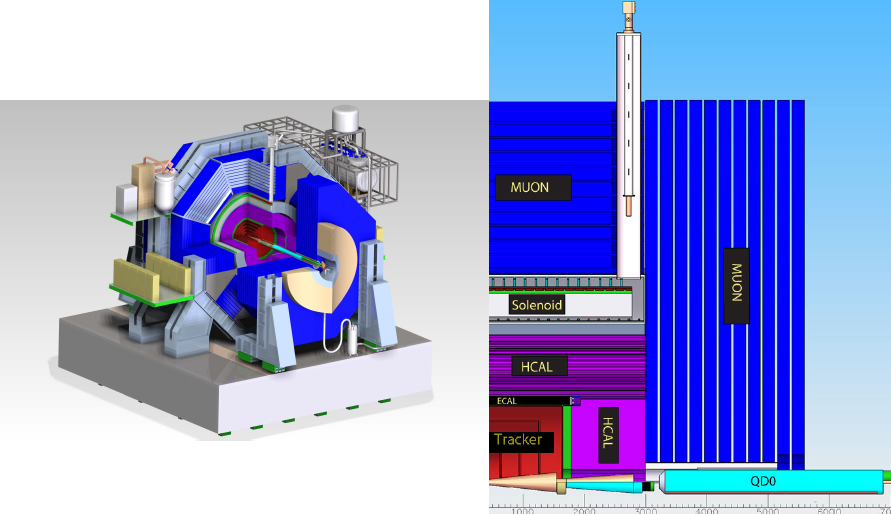
\includegraphics[width=1.0\textwidth]{ILC/figs/sid.png}
    \caption{Image artistique (à gauche) et vue en coupe d'un quadrant (à droite) du détecteur SiD.}
    \label{fig:sid-scheme}
  \end{center}
\end{figure}
Le deuxième concept de détecteur pour l'ILC est le Détecteur au Silicium (SiD)~\cite{detectorTDR}. La figure~\ref{fig:sid-scheme} présente une vue artistique du détecteur SiD et une vue en coupe montrant ses différents sous-détecteurs. La principale différence avec l'ILD est le trajectographe. En effet, à la place d'une TPC, des couches concentriques de silicium sont utilisées. Cette technologie permet d'obtenir une meilleure résolution spatiale sur chaque point de la trajectoire d'une trace. Cependant, le budget matière est plus important qu'avec une TPC. Ainsi, le rayon du trajectographe est plus faible que pour l'ILD. Afin d'obtenir un pouvoir de séparation suffisant, le champ magnétique est de 5 $T$ (contre 3.5 à 4 $T$ pour l'ILD). Le système de calorimètre est aussi basé sur des calorimètres ultra-granulaires pour appliquer des techniques de suivi de particules. 
\newpage
\section{Le programme de physique de l'ILC}
\label{sec.phys.program}
\begin{table}[!ht]
  \begin{center}
    \begin{tabular}{c|c|c|c}
      \rowcolor{black!20!white}Énergie & Réaction physique & Motivation \\
      \hline
      \rowcolor{black!5!white}$91~GeV$ & $e^+e^-~\rightarrow~Z$ & Mesure de précision électrofaible  \\
      \hline
      \rowcolor{black!5!white}$160~GeV$ & $e^+e^-~\rightarrow~WW$ & Masse du W  \\
      \hline
      \rowcolor{black!5!white}$250~GeV$ & $e^+e^-~\rightarrow~ZH$ & Couplages du Higgs  \\
      \hline
      \rowcolor{black!5!white}$350-400~GeV$ & $e^+e^-~\rightarrow~t\bar t$ & Couplages et masse du quark top  \\
      \rowcolor{black!5!white}$ $ & $e^+e^-~\rightarrow~WW$ & Couplages du W  \\
      \rowcolor{black!5!white}$ $ & $e^+e^-~\rightarrow~\nu\bar{\nu}H$ & Couplages du Higgs  \\
      \hline
      \rowcolor{black!5!white}$500~GeV$ & $e^+e^-~\rightarrow~f\bar f$ & Recherche d'un boson $Z'$  \\
      \rowcolor{black!5!white}$ $ & $e^+e^-~\rightarrow~t\bar tH$ & Couplages du Higgs au quark t  \\
      \rowcolor{black!5!white}$ $ & $e^+e^-~\rightarrow~ZHH$ & Auto-couplage du Higgs  \\
      \rowcolor{black!5!white}$ $ & $e^+e^-~\rightarrow~\bar{\chi}\bar{\chi}$ & Recherche de supersymétrie  \\
      %\rowcolor{black!5!white}$ $ & $e^+e\rightarrow~AH,H^+H^-$ & Recherche de nouveaux états du Higgs  \\
      \hline
      \rowcolor{black!5!white}$700-1000~GeV$ & $e^+e^-~\rightarrow~\nu\bar{\nu}HH$ & Auto-couplage du Higgs  \\
      %\rowcolor{black!5!white}$ $ & $e^+e^-~\rightarrow~\bar t\bar t^*$ & Recherche de supersymétrie  \\
      %\rowcolor{black!5!white} %$e^+e^-~\rightarrow~\nu\bar{\nu}t\bar t$ & composite Higgs and top L
      %$ $ & $e^+e^-~\rightarrow~‹¯‹V V composite Higgs sector L
    \end{tabular}
  \end{center}  
  \caption{Tableau récapitulatif des processus physiques majeurs qui seront étudiés en fonction de l'énergie dans le centre de masse \cite{physicsTDR}.}
  \label{tab.physic_summary}
\end{table}
Comme nous l'avons déjà précisé, un des intérêts majeurs d'un collisionneur linéaire est de pouvoir régler l'énergie dans le centre de masse. En principe, il est possible de parcourir toute la gamme d'énergie jusqu'à l'énergie maximum définie par la longueur des bras d'accélérateur principaux. Ils pourraient être allongés en cas d'augmentation du budget de l'expérience, motivée par l'opportunité de découvertes physiques. Un programme de physique, résumé dans le tableau~\ref{tab.physic_summary}, a été défini \cite{physicsTDR}:
\begin{itemize}
\item \textbf{91 et 160 GeV}: Ces énergies correspondent à la masse du boson Z et au seuil de la réaction $e^+e^-\rightarrow W^+W^-$. Ces études permettront d'améliorer d'un ordre de magnitude la précision des couplages du boson Z et de mesurer la masse du boson W avec une précision de l'ordre du $MeV$.
\begin{figure}[!h]
  \begin{center}
    \subfigure[]{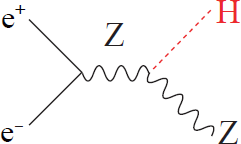
\includegraphics[width=.31\textwidth]{ILC/figs/z-hz.png}}
    \subfigure[]{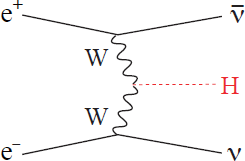
\includegraphics[width=.31\textwidth]{ILC/figs/ww-hnunu.png}}
    \subfigure[]{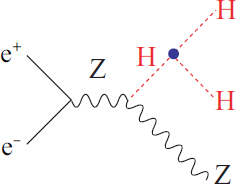
\includegraphics[width=.31\textwidth]{ILC/figs/z-zh-hh.png}}
    \caption{Diagramme de Feynman associé aux réactions $e^+e^-\rightarrow ZH$ (a), $e^+e^-\rightarrow \nu\bar{\nu}H$ (b) et $e^+e^-~\rightarrow~ZHH$ (c).}
     \label{fig:feynmanILC}
  \end{center}
\end{figure}
\item \textbf{250 GeV}: La réaction $e^+e^-\rightarrow ZH$ (voir figure~\ref{fig:feynmanILC}(a)) est une réaction très importante pour l'étude du nouveau boson de 125 $GeV$ récemment découvert au LHC. Que la nouvelle particule soit le boson de Higgs ou non, l'étude de cette réaction permettra de mesurer ses propriétés quelque soit son mode de désintégration. La section efficace de cette réaction est maximale à 250 $GeV$ comme le montre la figure~\ref{fig:hCross}.
\begin{figure}[!h]
  \begin{center}
    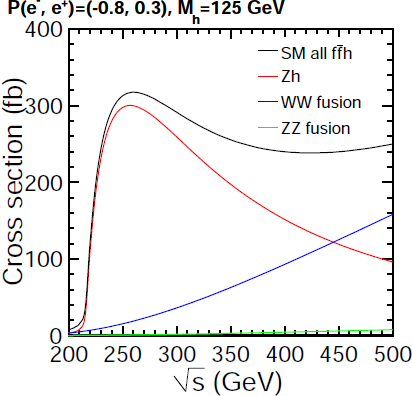
\includegraphics[width=.7\textwidth]{ILC/figs/hcross.png}
    \caption{Sections efficaces de production des processus $e^+e^-\rightarrow ZH$ et ceux associés aux fusions de bosons $W^+W^-$ ($e^+e^-~\rightarrow~\nu\bar{\nu}H$) et $ZZ$ ($e^+e^-~\rightarrow~e^+e^-H$) pour un boson de Higgs de 125 $GeV$ en fonction de l'énergie dans le centre de masse.}
     \label{fig:hCross}
  \end{center}
\end{figure}
\item \textbf{350-400 GeV}: Le seuil de production d'une paire de quark top se trouve autour de 350 $GeV$. La masse du quark top sera étudiée avec une précision attendue de l'ordre de 100 $MeV$. Dans cette gamme d'énergie, la section efficace de la réaction $e^+e^-~\rightarrow~\nu\bar{\nu}H$, devient significative. Ce processus, où le boson de Higgs est produit grâce à une fusion de deux bosons W (voir figure~\ref{fig:feynmanILC}(b)), devient le processus majeur de sa production à partir 450 $GeV$ (voir figure~\ref{fig:hCross}). Enfin, dans cette gamme d'énergie, la réaction $e^+e^-$ devient très sensible aux possibles modifications des couplages du modèle standard. Ainsi, une précision optimale de mesure des couplages du boson W, pourrait permettre de découvrir des nouveaux phénomènes physiques. 
\item \textbf{500 GeV}: Cette énergie correspond à l'énergie nominale de l'ILC. La luminosité nominale sera aussi atteinte à 500 $GeV$ ce qui permettra de poursuivre les mesures de précision décrites précédemment. En plus de ces mesures, les réactions $e^+e^-\rightarrow f\bar{f}$ (avec $f$ un quark ou un lepton) seront utilisées pour étudier des modèles au-delà du modèle standard (nouveau type d'interaction, structure interne des quarks et des leptons). L'auto-couplage du boson de Higgs sera aussi étudié grâce à la réaction $e^+e^-~\rightarrow~ZHH$ (voir figure~\ref{fig:feynmanILC}(c)). Enfin, à 500 $GeV$, une mesure du couplage du quark top au boson de Higgs à travers la réaction $e^+e^-~\rightarrow~t\bar tH$ devient possible (seuil à $\sqrt{s}\approx450~GeV$).
\item \textbf{700-1000 GeV}: Dans le cas d'une augmentation de l'énergie maximale de l'ILC (en doublant la taille des accélérateurs principaux), de nouvelles mesures sur l'auto-couplage du Higgs, et de son couplage au quark top deviennent envisageable. Des recherches au-delà du modèle standard seront aussi entreprises dans cette gamme d'énergie. 
\end{itemize}

Ce programme (non exhaustif) sera amené à évoluer en fonction de la situation en physique des particules lorsque l'ILC sera opérationnel. En effet, même si les analyses de données au LHC à 7 et 8 $TeV$ n'indiquent pas la présence de nouvelle physique, les futures prises de données à 13 et 14 $TeV$ pourraient changer la donne. Une part importante du programme de physique de l'ILC est dédiée aux mesures de précision relatives au nouveau boson de 125 $GeV$ découvert par le LHC en 2012. Ces mesures de précision motivent aussi plusieurs études d'accélérateurs électron-positon. 
\section{Les autres concepts de collisionneur leptonique}
\label{sec.clic}
En parallèle des études pour l'ILC, d'autres projets de collisionneurs électron-positon sont imaginés. Le premier projet est le Collisionneur Linéaire Compact CLIC \cite{clicAcc}, développé au CERN, avec une énergie dans le centre de masse entre 1 et 3 $TeV$. Pour atteindre de telles énergies tout en conservant une taille d'expérience raisonnable, il est nécessaire d’obtenir un gradient moyen d'accélération de l'ordre de 100 $MV/m$ (31.5 $MV/m$ pour l'ILC). Il n'est pas possible d'atteindre ce gradient avec les cavités supraconductrices. Ainsi, une autre technique d'accélération est développée pour ce collisionneur. Cette technique utilise deux faisceaux. Un premier faisceau d'électron de grande intensité mais de faible énergie, transfère son énergie au faisceau principal de faible intensité. Avec cette technique, un collisionneur pouvant atteindre une énergie dans le centre de masse de 3 $TeV$ aurait une longueur d'environ 48 $km$. 

Deux projets de collisionneur électron-positon circulaire sont aussi à l'étude: le FCC (Future Circular Collider) \cite{fcc-ee} et le CEPC (Circular Electron Positron Collider) \cite{cepc}. Le premier est un accélérateur de 80 à 100 $km$ de circonférence avec une énergie dans le centre de masse de 90 à 400 $GeV$. Cet accélérateur serait installé dans la région du CERN. Le deuxième, de 50 à 70 $km$ de circonférence, serait construit en Chine, avec une énergie dans le centre de masse d'environ 250 $GeV$. Le principal intérêt des collisionneurs leptoniques circulaires est la luminosité qui peut être beaucoup plus élevée que pour les collisionneurs linéaires, comme le montre la figure~\ref{fig:fccLumi}.
De plus, contrairement au collisionneur linéaire, plusieurs points d'interaction sont possibles. Enfin, la construction de telles infrastructures permettraient de préparer le futur (assez lointain). Ces infrastructures pourront être réutilisées pour la construction de collisionneurs hadroniques avec une énergie dans le centre de masse entre 50 et 100 $TeV$. 
\begin{figure}[!h]
  \begin{center}
    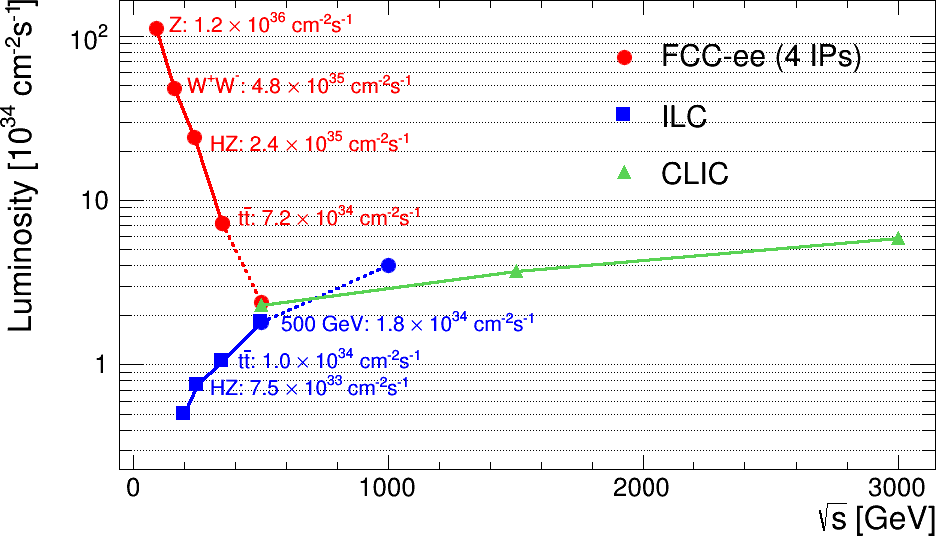
\includegraphics[width=1.0\textwidth]{ILC/figs/fcc_ilc_clic_lumi.png}
    \caption{Luminosité instantanée en fonction de l'énergie dans le centre de masse pour les trois accélérateurs FCC, ILC et CLIC.}
    \label{fig:fccLumi}
  \end{center}
\end{figure}
